\documentclass[aspectratio=169,10pt]{beamer}

\usetheme[block=fill,progressbar=foot,background=light]{metropolis}   
\setbeamercolor{background canvas}{bg=white}
\usepackage{appendixnumberbeamer}

\title{Introduction au DevOps}
\subtitle{Docker}
\date{12 Septembre 2025}
\author{Jolan PHILIPPE}
\institute{Université d'Orléans}

\usepackage{graphicx}
%\usepackage{cite}
\usepackage{subcaption}
\usepackage{lmodern}
\usepackage{hyperref}
\usepackage{array}
\usepackage{multirow}
%\usepackage[table]{xcolor}
\usepackage{mathabx}
\usepackage{amsmath}
\usepackage{amssymb}
\usepackage{wrapfig}
\usepackage{fancyhdr}
\usepackage{url}
\usepackage{listings}
\usepackage{minted}
\usepackage{fontawesome}
\usepackage{tikz}
\usepackage{hyperref}
\usetikzlibrary{automata, positioning, matrix, fit}
\usetikzlibrary{arrows.meta,calc,decorations.markings,math}
\usetikzlibrary{shadows.blur}
\usetikzlibrary{decorations.pathreplacing, fit}
\usetikzlibrary{shapes,arrows}
\usepackage{flushend}
\usepackage{ifthen}
\newboolean{showtodos}

% ----------------------------------------
% COLORS
\definecolor{gray}{rgb}{0.5,0.5,0.5}
\definecolor{ashgrey}{rgb}{0.7, 0.75, 0.71}
\definecolor{battleshipgrey}{rgb}{0.52, 0.52, 0.51}
\definecolor{aliceblue}{rgb}{0.94, 0.97, 1.0}
\definecolor{mauve}{rgb}{0.58,0,0.82}
\definecolor{auburn}{rgb}{0.43, 0.21, 0.1}
\definecolor{babyblue}{rgb}{0.54, 0.81, 0.94}
\definecolor{amaranth}{rgb}{0.9, 0.17, 0.31}
\definecolor{bleudefrance}{rgb}{0.19, 0.55, 0.93}
\definecolor{atomictangerine}{rgb}{1.0, 0.6, 0.4}
\definecolor{beaublue}{rgb}{0.74, 0.83, 0.9}
\definecolor{dkviolet}{rgb}{0.9, 0.17, 0.31}
\definecolor{dkgreen}{rgb}{0.0, 0.42, 0.24}
\definecolor{ltblue}{rgb}{0.0, 0.75, 1.0}
\definecolor{dkblue}{rgb}{0.2, 0.2, 0.6}
\definecolor{dkred}{rgb}{0.8, 0.0, 0.0}
\definecolor{byzantine}{rgb}{0.74, 0.2, 0.64}
% ----------------------------------------



\usepackage[textwidth=17mm]{todonotes}
\newcommand{\instructions}[1]{
	\todo[color=black!20,inline,size=\small]{#1}
}
\newcommand{\customtodo}[4]{
\ifthenelse{\boolean{showtodos}} { 
	\todo[color=#2,inline,size=\small]{
		\ifx&#3&
		\textbf{#1} #4
		\else
		\textbf{#1$\Rightarrow$#3} #4
		\fi
	}
 } 
}{}

\newcommand{\jolan}[2][]{\customtodo{Jolan}{pink!40}{#1}{#2}}
\newcommand{\antoine}[2][]{\customtodo{Antoine}{red!40}{#1}{#2}}
\newcommand{\helene}[2][]{\customtodo{Helene}{orange!40}{#1}{#2}}
\newcommand{\issam}[2][]{\customtodo{Issam}{green!40}{#1}{#2}}
\newcommand{\charles}[2][]{\customtodo{Charles}{blue!40}{#1}{#2}}

\newcommand{\tmp}[1][]{\customtodo{To remove}{gray}{#1}}

\usepackage{xspace}
\newcommand{\ie}[0]{{\em i.e.},\xspace}
\newcommand{\vs}[0]{{\em vs.}\xspace}
\newcommand{\eg}[0]{{\em e.g.},\xspace}
\newcommand{\etal}[0]{{\em et al.}\xspace}
\newcommand{\wrt}[0]{{\em w.r.t.}\xspace}
\newcommand{\aka}[0]{{\em a.k.a.}\xspace}
\newcommand{\via}[0]{{\em via}\xspace}

% ----------------------------------------

\lstdefinestyle{goalstyle}{
  basicstyle=\scriptsize\itshape,
  xleftmargin=1em,
  literate={::=}{$::=$}{2},
  keywords={behaviors,ports,components,forall,component,behavior,port,status}
}

\lstdefinelanguage{MiniZinc}{
numberstyle=\tiny\color{gray},
% Anything betweeen $ becomes LaTeX math mode
mathescape=true,
% Comments may or not include Latex commands
texcl=false,
% Vernacular commands
morekeywords=[1]{ann, annotation, any, array, assert,
        bool,
        constraint,
        else, elseif, endif, enum, exists,
        float, forall, function,
        if, in, include, int,
        list,
        minimize, maximize,
        of, op, output,
        par, predicate,
        record,
        set, solve, string,
        test, then, tuple, type,
        var,
        where,
        %% MiniZinc functions
        %%
        abort, abs, acosh, array_intersect, array_union,
        array1d, array2d, array3d, array4d, array5d, array6d, asin, assert, atan,
        bool2int,
        card, ceil, combinator, concat, cos, cosh,
        dom, dom_array, dom_size, dominance,
        exp,
        fix, floor,
        index_set, index_set_1of2, index_set_2of2, index_set_1of3, index_set_2of3, index_set_3of3,
        int2float, is_fixed,Yaml
        join,
        lb, lb_array, length, let, ln, log, log2, log10,
        min, max,
        pow, product,
        round,
        set2array, show, show_int, show_float, sin, sinh, sqrt, sum,
        tan, tanh, trace,
        ub, and ub_array,
        %% Search keywords
        bool_search, int_search, seq_search, priority_search,
        %% MiniSearch keywords
        minisearch, search, while, repeat, next, commit, print, post, sol, scope, time_limit, break, fail},
numbers=left,
% Gallina
morekeywords=[2]{Array},
% Spaces are not displayed as a special character
showstringspaces=false,
% String delimiters
morestring=[b]",
morestring=[d]',
% Size of tabulations
tabsize=2,
% Enables ASCII chars 128 to 255
extendedchars=false,
% Case sensitivity
sensitive=true,
% Automatic breaking of long lines
breaklines=false,
% Default style fors listings
basicstyle=\footnotesize,
% Position of captions is bottom
captionpos=b,
% flexible columns
basewidth={2em, 0.5em},
columns=[l]flexible,
% Style for (listings') identifiers
identifierstyle={\ttfamily\color{black}},
% Style for declaration keywords
keywordstyle=[1]{\ttfamily\bfseries\color{dkviolet}},
% Style for gallina keywords
keywordstyle=[2]{\ttfamily\bfseries\color{dkgreen}},
% Style for strings
stringstyle=\ttfamily,
% Style for comments
commentstyle={\ttfamily\itshape\color{dkgreen}},
%moredelim=**[is][\ttfamily\color{red}]{/&}{&/},
literate=
  {forall}{{\color{dkgreen}{$\forall$}}}1
{exists}{{$\exists$}}1
{<-}{{$\leftarrow$}}1
{=>}{{$\Rightarrow$}}1
%{==}{{\code{==}}}1
%{==>}{{\code{==>}}}1
%    {:>}{{\code{:>}}}1
{->}{{$\rightarrow$}}1
{<-->}{{$\longleftrightarrow$}}1
{<->}{{$\leftrightarrow$}}1
{<==}{{$\leq$}}1
{\#}{{$^\star$}}1
{\\o}{{$\circ$}}1
%    {\@}{{$\cdot$}}1 
{\/\\}{{$\wedge$}}1
{\\\/}{{$\vee$}}1
%{++}{{\code{++}}}1
{~}{{\ }}1
{\@\@}{{$@$}}1
{\\mapsto}{{$\mapsto$}}1
{\\hline}{{\rule{\linewidth}{0.5pt}}}1
%
}[keywords,comments,strings]
\lstdefinestyle{mznstyle}{
  language=MiniZinc,
}
% ----------------------------------------
\lstdefinelanguage{MyPython}{
morekeywords=[1]{def, if, while, return, not},
morekeywords=[5]{get_messages, infer_constraints, plan_inference, infer_messages, bhv_inference, send_messages, allAcked, send_ack, ack, global_ack},
keywordstyle=[5]{\ttfamily\bfseries\color{purple}},
tabsize=2,
numbers=left,
numberstyle=\tiny\color{gray},
breaklines=true,
basicstyle=\footnotesize,
% literate= 
% {act_c}{{$act_c$}}1
% {Gbhv}{{$\Gamma bhv$}}1
% {Gfinal}{{$\Gamma final$}}1,
% {Gbhv_c}{{$\Gamma bhv_{c}$}}1
% {Gport_c}{{$\Gamma port_{c}$}}1
% {Gfinal_c}{{$\Gamma final_{c}$}}1
}
\lstdefinestyle{pythonstyle}{language=MyPython}
\lstMakeShortInline[language=MyPython]"

\newfloat{Model}{t}{lom}
\newcommand{\constraint}[1]{\textnormal{\textsc{#1}}}
\newcommand{\Regular}{\constraint{Regular}}
\newcommand{\CostRegular}{\constraint{CostRegular}}
\newcommand{\Count}{\constraint{Count}}
\newcommand{\Element}{\constraint{Element}}
\newcommand{\Sum}{\constraint{Sum}}

%------------------------------------------------------
\definecolor{codegreen}{rgb}{0,0.6,0}
\definecolor{codegray}{rgb}{0.5,0.5,0.5}
\definecolor{codepurple}{rgb}{0.58,0,0.82}
\definecolor{backcolour}{rgb}{0.95,0.95,0.92}
\lstdefinestyle{mystyle}{
    commentstyle=\color{codegreen},
    keywordstyle=\color{purple},
    tabsize=2,
    numbers=left,
    numberstyle=\tiny\color{gray},
    stringstyle=\color{codepurple},
    breaklines=true,
    basicstyle=\tiny
}


\definecolor{keywords}{RGB}{255,0,90}
\definecolor{comments}{RGB}{0,0,113}
\definecolor{red}{RGB}{160,0,0}
\definecolor{green}{RGB}{0,150,0}
\definecolor{backcolour}{rgb}{0.95,0.95,0.95}
\DeclareCaptionFont{white}{\color{white}}
\DeclareCaptionFont{gray}{\color{gray}}
\DeclareCaptionFormat{listing}{\colorbox{backcolour}{\parbox{\linewidth}{#1#2#3}}}
\captionsetup[lstlisting]{format=listing}%,labelfont=white,textfont=white}
\lstdefinestyle{mystyle}{
    tabsize=2,
    numberstyle=\tiny\color{gray},
    breaklines=true,
    numbers=left,
    backgroundcolor=\color{white},
    numbersep=5pt,
    keywordstyle=\color{keywords},
    commentstyle=\color{comments},
    stringstyle=\color{blue},
    showstringspaces=false,
    identifierstyle=\color{green},
    basicstyle=\scriptsize\ttfamily,
    numberstyle=\tiny\color{gray},
}

\lstdefinestyle{mysmallstyle}{
    tabsize=2,
    numberstyle=\tiny\color{gray},
    breaklines=true,
    numbers=left,
    backgroundcolor=\color{white},
    numbersep=5pt,
    keywordstyle=\color{keywords},
    commentstyle=\color{comments},
    stringstyle=\color{blue},
    showstringspaces=false,
    identifierstyle=\color{green},
    basicstyle=\scriptsize\ttfamily,
    numberstyle=\tiny\color{gray},
}

\lstdefinestyle{yaml}{
     basicstyle=\color{black}\scriptsize,
     keywords =[1]{behaviors, components, connections},
    keywordstyle=[1]{\color{blue}\scriptsize}, 
     rulecolor=\color{black},
     string=[s]{'}{'},
     stringstyle=\color{blue},
     comment=[l]{:},
     commentstyle=\color{black},
     morecomment=[l]{-}
 }

\usepackage{pifont,utfsym}
\newcommand{\cmark}{\ding{51}}
\newcommand{\xmark}{\ding{55}}
\newcommand{\OKmark}{{\color{green}\cmark}}
\newcommand{\KOmark}{{\color{red}\xmark}}



% \usetikzlibrary{positioning, arrows.meta, decorations.pathreplacing, fit}
% \pgfarrowsdeclare{lollipop}{lollipop}{
%     \pgfsetlinewidth{0.7pt}
%     \pgfarrowsleftextend{0pt}
%     \pgfarrowsrightextend{2pt}
% }{
%     \pgfpathcircle{\pgfpoint{0pt}{0pt}}{2pt}
%     \pgfusepathqfillstroke
% }
% \pgfarrowsdeclare{socket}{socket}{
%     \pgfarrowsleftextend{2pt}
%     \pgfarrowsrightextend{2pt}
% }{
%     \pgfsetlinewidth{0.7pt}
%     \pgfpathmoveto{\pgfqpoint{3pt}{-3pt}}
%     \pgfpatharc{270}{90}{3pt}
%     \pgfusepathqstroke
% }

% % Define styles for lollipop and socket arrows
% \tikzset{
%   lollipop/.style={
%     -{lollipop}
%   },
%   socket/.style={
%     -{socket}
%   }
% }





% Define a new arrow tip for the lollipop (filled circle)
\pgfarrowsdeclare{lollipop}{lollipop}{
    \pgfsetlinewidth{0.7pt}
    \pgfarrowsleftextend{0pt}
    \pgfarrowsrightextend{2pt}
}{
    \pgfpathcircle{\pgfpoint{0pt}{0pt}}{2pt}
    \pgfusepathqfillstroke
}

% Define a new arrow tip for the socket (reversed C)
\pgfarrowsdeclare{socket}{socket}{
    \pgfarrowsleftextend{2pt}
    \pgfarrowsrightextend{2pt}
}{
    \pgfsetlinewidth{0.7pt}
    \pgfpathmoveto{\pgfqpoint{3pt}{-3pt}}
    \pgfpatharc{270}{90}{3pt}
    \pgfusepathqstroke
}

% Define styles for lollipop and socket arrows
\tikzset{
  lollipop/.style={
    -{lollipop}
  },
  socket/.style={
    -{socket}
  }
}

\newcommand{\simpleprovideuse}[3][1cm]{%
    \path (#2) -- (#3) coordinate[pos=0.5] (mid#2#3);
    \draw[-{lollipop}] (#2) -- (mid#2#3);
    \draw[-{socket}] (#3) -- (mid#2#3);
}

\newcommand{\provideuse}[3][1cm]{
    % Usage :
    %   \provideuse{src}{target}
    % Example:
    %   \node[draw, circle] (A) {A};
    %   \node[draw, circle] (B) {B};
    %   \provideuse{A}{B}
    \path (#2) -- (#3) coordinate[pos=0.5] (mid#2#3);
    \path (#2) -- (mid#2#3) coordinate[pos=0.5] (q1#2#3);
    \path (mid#2#3) -- (#3) coordinate[pos=0.5] (q3#2#3);
    \draw[-{lollipop}] (#2) -- (q1#2#3);
    \draw[-{lollipop}] (mid#2#3) -- (q3#2#3);
    \draw[-{socket}] (#3) -- (q3#2#3);
    \draw[-{socket}] (q3#2#3) -- (q1#2#3);
}

\newcommand{\provideusetwolabels}[5][1cm]{%
    % Usage :
    %   \provideusetwolabels{src}{target}
    % Example:
    %   \node[draw, circle] (A) {A};
    %   \node[draw, circle] (B) {B};
    %   \provideusetwolabels{A}{B}{provide}{use}
    \path (#2) -- (#3) coordinate[pos=0.5] (mid#2#3);
    \path (#2) -- (mid#2#3) coordinate[pos=0.5] (q1#2#3);
    \path (mid#2#3) -- (#3) coordinate[pos=0.5] (q3#2#3);
    \draw[-{lollipop}] (#2) --  node[midway, above, xshift=0.08cm] {\tiny #4} (q1#2#3);
    \draw[-{lollipop}] (mid#2#3) -- (q3#2#3);
    \draw[-{socket}] (#3) -- node[midway, below, xshift=-0.4cm] { \tiny #5} (q3#2#3);
    \draw[-{socket}] (q3#2#3) -- (q1#2#3);
}

\newcommand{\provideusesinglelabel}[4][1cm]{%
    % Usage :
    %   \provideusesinglelabel{src}{target}
    % Example:
    %   \node[draw, circle] (A) {A};
    %   \node[draw, circle] (B) {B};
    %   \provideusesinglelabel{A}{B}{relation}
    \path (#2) -- (#3) coordinate[pos=0.5] (mid#2#3);
    \path (#2) -- (mid#2#3) coordinate[pos=0.5] (q1#2#3);
    \path (mid#2#3) -- (#3) coordinate[pos=0.5] (q3#2#3);
    \draw[-{lollipop}] (#2) -- (q1#2#3);
    \draw[-{lollipop}] (mid#2#3) -- (q3#2#3);
    \draw[-{socket}] (#3) -- (q3#2#3);
    \draw[-{socket}] (q3#2#3)  -- node[midway, above] {\scriptsize #4} (q1#2#3);
}

\usepackage{pifont,utfsym}
\newcommand{\cmark}{\ding{51}}
\newcommand{\xmark}{\ding{55}}
\newcommand{\okmark}{\textbf{\color{green}\faCheck}}
\newcommand{\komark}{\textbf{\color{red}\faTimes}}
\newcommand{\midmark}{\textbf{\color{orange}$\sim$}}
\renewcommand{\OKmark}{\okmark~}
\newcommand{\OKOKmark}{\okmark\okmark~}
\renewcommand{\KOmark}{\komark~}
\newcommand{\MIDmark}{\midmark~}

\begin{document}

\begin{frame}
    \titlepage 
\end{frame}
% -----------------

\begin{frame}{Les rôles des outils d'IaC}

\hspace*{-0.7cm}
\begin{tikzpicture}

    % \node[] (commit) {Commit Code};

\node[] (packaging) {
    \begin{tabular}{c}
    \textbf{Management}\\
    \textbf{d'application}
    \end{tabular}
    };
\node[below=0cm of packaging] (packagingL) {
    \begin{tabular}{c}
    \small Customiser, configurer\\
    \small tester l'application\\
    \small et la conteneuriser\\
    \small 
    \end{tabular}
};
\node[right=0.8cm of packaging] (provisioning) {
    \begin{tabular}{c}
    \textbf{Provisionnement} \\ 
    \textbf{d'infrastructure}
    \end{tabular}
};
\node[below=0cm of provisioning] (provisioningL) {
    \begin{tabular}{c}
    \small Demander ressources\\
    \small physiques ou virtuelles;\\
    \small configurer le réseau;\\
    \small et règles sécurité
    \end{tabular}
};
    
\node[right=0.8cm of provisioning] (configmanagement) {
    \begin{tabular}{c}
    \textbf{Installation et}\\
    \textbf{Configuration}
    \end{tabular}
};
\node[below=0cm of configmanagement] (configmanagementL) {
    \begin{tabular}{c}
    \small Installer les services\\
    \small (app + deps)\\
    \small configurer les services;\\
    \small et les intégrer
    \end{tabular}
};

    % -------

\node[right=0.8cm of configmanagement] (orchestration) {
\begin{tabular}{c}
\textbf{Orchestration}\\
\textbf{de cycle de vie}
\end{tabular}
};
\node[below=0cm of orchestration] (orchestrationL) {
\begin{tabular}{c}
\small Upgrades auto;\\
\small Backup et recovery;\\
\small Surveillance;\\
\small Passage à l'échelle
\end{tabular}
};

\node[rectangle, draw, fit=(provisioning) (provisioningL), dkblue, line width=2pt](){};
    
\end{tikzpicture}

\url{https://www.docker.com/blog/docker-for-devops/}

\end{frame}

% -----------------
\section{Un conteneur c'est quoi ?}
% -----------------


\begin{frame}{A propos du kernel Linux}

Le kernel c'est le cœur d'un système d'exploitation (OS)

\begin{itemize}
    \item C'est une partie de l'OS toujours chargé en mémoire.
    \item Il contrôle les ressources physiques, ou hardware, (e.g., I/O, mémoire, cryptographie, CPU) en utilisant des pilotes, ou drivers.
    \item Il arbitre les conflits et la concurrence entre les processus.
    \item Il optimise l'utilisation de ressources (e.g., cache, mémoire, CPU, système de fichiers, réseau)
\end{itemize}

Le kernel est l'un des premiers programmes chargé au démarrage.

\end{frame}

% -----------------

\begin{frame}{Comparaison à gros grains entre les VMs et les conteneurs}

\begin{tikzpicture}

    \node[] (vm1tmp) {VM 1};
    \node[minimum height=0.6cm, minimum width=2cm, below=0.15cm of vm1tmp] (appBVMtmp) {};
    \node[minimum height=0.6cm, rounded corners=2, minimum width=2cm, below=0.15cm of appBVMtmp] (appAVMtmp) {};
    \node[minimum height=0.6cm, rounded corners=2, minimum width=2cm, below=0.3cm of appAVMtmp] (binlibsVM1tmp) {};
    \node[minimum height=0.6cm, minimum width=2cm, below=0.15cm of binlibsVM1tmp] (os1tmp) {};
    
    \node[draw, fit=(vm1tmp)(os1tmp), inner sep=3pt, fill=brightlavender] (vm1box) {};

    \node[] (vm1) {VM 1};
    \node[draw, rectangle, minimum height=0.6cm, rounded corners=2, below=0.15cm of vm1, minimum width=2cm, fill=apricot] (appBVM) {app B};
    \node[draw, rectangle, minimum height=0.6cm, rounded corners=2, minimum width=2cm, below=0.15cm of appBVM, fill=apricot] (appAVM) {app A};
    \node[draw, rectangle, minimum height=0.6cm, rounded corners=2, minimum width=2cm, below=0.3cm of appAVM, fill=celadon] (binlibsVM1) {bin/libs};
    \node[draw, rectangle, minimum height=0.6cm, rounded corners=2, minimum width=2cm, below=0.15cm of binlibsVM1, fill=celadon] (os1) {guest OS};

    % ------------------------------------

     \node[right=1.5cm of vm1tmp] (vm2tmp) {VM 2};
    \node[minimum height=0.6cm, minimum width=2cm, below=0.15cm of vm2tmp] (appDVMtmp) {};
    \node[minimum height=0.6cm, rounded corners=2, minimum width=2cm, below=0.15cm of appDVMtmp] (appCVMtmp) {};
    \node[minimum height=0.6cm, rounded corners=2, minimum width=2cm, below=0.3cm of appCVMtmp] (binlibsVM2tmp) {};
    \node[minimum height=0.6cm, minimum width=2cm, below=0.15cm of binlibsVM2tmp] (os2tmp) {};
    
    \node[draw, fit=(vm2tmp)(os2tmp), inner sep=3pt, fill=brightlavender] (vm2box) {};

    \node[right=1.5cm of vm1] (vm2) {VM 2};
    \node[draw, rectangle, minimum height=0.6cm, rounded corners=2, below=0.15cm of vm2, minimum width=2cm, fill=apricot] (appDVM) {app D};
    \node[draw, rectangle, minimum height=0.6cm, rounded corners=2, minimum width=2cm, below=0.15cm of appDVM, fill=apricot] (appCVM) {app C};
    \node[draw, rectangle, minimum height=0.6cm, rounded corners=2, minimum width=2cm, below=0.3cm of appCVM, fill=celadon] (binlibsVM2) {bin/libs};
    \node[draw, rectangle, minimum height=0.6cm, rounded corners=2, minimum width=2cm, below=0.15cm of binlibsVM2, fill=celadon] (os2) {guest OS};
    
    % ------------------------------------
    \node[fit=(vm2box)(vm1box), inner sep=3pt] (vmboxes) {};
    \node[draw, below=0.05cm of vmboxes, minimum height=0.6cm, rounded corners=2, minimum width=4.8cm, fill=blizzardblue] (vmhypervisor) {Hypervisor};
    \node[draw, below=0.05cm of vmhypervisor, minimum height=0.6cm, rounded corners=2, minimum width=4.8cm, fill=celadon] (vmos) {host OS};
    \node[below=0.2cm of vmos] (vmlabel) {bare metal machine};
    \node[draw, fit=(vm2box)(vm1box)(vmlabel), inner sep=3pt] (baremetalmachine) {};
    \node[below=0.2cm of baremetalmachine] () {\large VMs avec un hyperviseur};
    
    % ------------------------------------
    
    \node[minimum height=0.6cm, minimum width=2cm, below=-0.18cm of appCVM, xshift=2.75cm] (appAconttmp) {};
    \node[minimum height=0.6cm, minimum width=2cm, above=0.15cm of appAconttmp] (cont1tmp) {};
    \node[minimum height=0.6cm, minimum width=2cm, below=0.15cm of appAconttmp] (binlibscont1tmp) {};
    \node[minimum height=0.6cm, minimum width=2cm, below=0.15cm of binlibscont1tmp] (os1conttmp) {};
    \node[draw, fit=(cont1tmp)(os1conttmp), inner sep=3pt, fill=brightlavender] (cont1box) {};
    \node[draw, rectangle, minimum height=0.6cm, rounded corners=2, minimum width=2cm, below=-0.18cm of appCVM, xshift=2.75cm, fill=apricot] (appAcont) {app A};
    \node[minimum height=0.6cm, rounded corners=2, minimum width=2cm, above=0.15cm of appAcont] (cont1) {container 1};
    \node[draw, rectangle, minimum height=0.6cm, rounded corners=2, minimum width=2cm, below=0.15cm of appAcont, fill=celadon] (binlibscont1) {bin/libs};
    \node[draw, rectangle, minimum height=0.6cm, rounded corners=2, minimum width=2cm, below=0.15cm of binlibscont1, fill=celadon] (os1cont) {\footnotesize minimal OS};

    
    \node[minimum height=0.6cm, minimum width=2cm, right=0.3cm of appAcont] (appBconttmp) {};
    \node[minimum height=0.6cm, minimum width=2cm, above=0.15cm of appBconttmp] (cont2tmp) {};
    \node[minimum height=0.6cm, minimum width=2cm, below=0.15cm of appBconttmp] (binlibscont2tmp) {};
    \node[minimum height=0.6cm, minimum width=2cm, below=0.15cm of binlibscont2tmp] (os2conttmp) {};
    \node[draw, fit=(cont2tmp)(os2conttmp), inner sep=3pt, fill=brightlavender] (cont2box) {};
    \node[draw, rectangle, minimum height=0.6cm, rounded corners=2, minimum width=2cm,  right=0.3cm of appAcont, fill=apricot] (appBcont) {app B};
    \node[minimum height=0.6cm, rounded corners=2, minimum width=2cm, above=0.15cm of appBcont] (cont2) {container 2};
    \node[draw, rectangle, minimum height=0.6cm, rounded corners=2, minimum width=2cm, below=0.15cm of appBcont, fill=celadon] (binlibscont2) {bin/libs};
    \node[draw, rectangle, minimum height=0.6cm, rounded corners=2, minimum width=2cm, below=0.15cm of binlibscont2, fill=celadon] (os2cont) {\footnotesize minimal OS};

     
    \node[minimum height=0.6cm, minimum width=2cm, right=0.3cm of appBcont] (appCconttmp) {};
    \node[minimum height=0.6cm, minimum width=2cm, above=0.15cm of appCconttmp] (cont3tmp) {};
    \node[minimum height=0.6cm, minimum width=2cm, below=0.15cm of appCconttmp] (binlibscont3tmp) {};
    \node[minimum height=0.6cm, minimum width=2cm, below=0.15cm of binlibscont3tmp] (os3conttmp) {};
    \node[draw, fit=(cont3tmp)(os3conttmp), inner sep=3pt, fill=brightlavender] (cont3box) {};
    \node[draw, rectangle, minimum height=0.6cm, rounded corners=2, minimum width=2cm,  right=0.3cm of appBcont, fill=apricot] (appCcont) {app C};
    \node[minimum height=0.6cm, rounded corners=2, minimum width=2cm, above=0.15cm of appCcont] (cont3) {container 3};
    \node[draw, rectangle, minimum height=0.6cm, rounded corners=2, minimum width=2cm, below=0.15cm of appCcont, fill=celadon] (binlibscont3) {bin/libs};
    \node[draw, rectangle, minimum height=0.6cm, rounded corners=2, minimum width=2cm, below=0.15cm of binlibscont3, fill=celadon] (os3cont) {\footnotesize minimal OS};

     
    \node[minimum height=0.6cm, minimum width=2cm, right=0.3cm of appCcont] (appDconttmp) {};
    \node[minimum height=0.6cm, minimum width=2cm, above=0.15cm of appDconttmp] (cont4tmp) {};
    \node[minimum height=0.6cm, minimum width=2cm, below=0.15cm of appDconttmp] (binlibscont4tmp) {};
    \node[minimum height=0.6cm, minimum width=2cm, below=0.15cm of binlibscont4tmp] (os4conttmp) {};
    \node[draw, fit=(cont4tmp)(os4conttmp), inner sep=3pt, fill=brightlavender] (cont4box) {};
    \node[draw, rectangle, minimum height=0.6cm, rounded corners=2, minimum width=2cm,  right=0.3cm of appCcont, fill=apricot] (appDcont) {app D};
    \node[minimum height=0.6cm, rounded corners=2, minimum width=2cm, above=0.15cm of appDcont] (cont4) {container 4};
    \node[draw, rectangle, minimum height=0.6cm, rounded corners=2, minimum width=2cm, below=0.15cm of appDcont, fill=celadon] (binlibscont4) {bin/libs};
    \node[draw, rectangle, minimum height=0.6cm, rounded corners=2, minimum width=2cm, below=0.15cm of binlibscont4, fill=celadon] (os4cont) {\footnotesize minimal OS};

    \node[fit=(cont1box) (cont4box)] (allcontbox) {};
    
    \node[draw, below=0.05cm of allcontbox, minimum height=0cm, rounded corners=2, minimum width=9.2cm, fill=blizzardblue] (conthypervisor) {\small container engine};
    \node[draw, below=0.05cm of conthypervisor, minimum height=0.6cm, rounded corners=2, minimum width=9.2cm, fill=celadon] (contos) {host OS};
    
    \node[below=0.0cm of contos] (allcontL) {bare metal machine};
    \node[draw, rectangle, fit=(allcontbox) (allcontL), inner sep=3pt] (containers) {};
    
    \node[below=0.2cm of allcontL] () {\large Containers};
    
\end{tikzpicture}

\end{frame}

% -----------------

\begin{frame}{Conteneurs}

\begin{alertblock}{Avantages des conteneurs}
   \begin{itemize}
       \item Isolation
       \item Portabilité
       \item Limitations des ressources dupliquées
       \item Impact limité sur les performances
       \item Démarrage rapide
   \end{itemize} 
   Le modèle est différent et la façon dont les applications sont déployées est différente !
\end{alertblock}

\end{frame}

% -----------------

\section{Que se cache-t-il dessous ?}

% -----------------

\begin{frame}{Un peu plus à propos de Linux}

Dans Unix/Linux, tout est fichier : une fichier, un dossier, un 
périphérique, etc.

\begin{alertblock}{Système de fichiers}
   \begin{itemize}
       \item Organisation des fichiers hierarchique sous la forme d'un arbre
       \item \texttt{\textbf{/}} est \alert{la racine du système de fichiers}
       \item \texttt{\textbf{/sys}} contient les fichiers du système
       \item \texttt{\textbf{/etc}} contient les fichiers de configuration et les scripts
       \item \texttt{\textbf{/media}} contient les partitions de disques, périphériques, etc.
       \item etc.
   \end{itemize} 
\end{alertblock}

    \alert{Un conteneur est aussi un ensemble de fichiers}

\end{frame}

% -----------------

\begin{frame}{Images}

Une image de conteneur est une archive de fichiers, incluant:

\begin{itemize}
   \item une racine de système de fichiers
   \item des bibliothèques, des packages, etc. (i.e., des dépendances)
   \item l'application, ou le service, à démarre
   \item etc.
\end{itemize} 

L'image contient l'environnement requis pour exécuter l'application ou le service sur le noyau hôte.

\end{frame}
% -----------------

\begin{frame}{Portabilité des images}

Cet environnement est \alert{portable} d'un hôte à un autre, si un kernel compatible est présent (\alert{WSL2 sur Windows}, ou \alert{VM sur MacOS})

\vspace{0.5cm}

\alert{Attention}: La limite, c’est l’architecture matérielle : par exemple une image construite pour amd64 ne tournera pas nativement sur un hôte arm64 (Mac M1/M2) sans émulation (e.g., qemu).


\end{frame}

% -----------------

\begin{frame}{Registre d'images}

 \begin{itemize}
    \item Les images Docker sont stockées dans des \textbf{registres} (e.g., \textit{Docker Hub} \url{https://hub.docker.com/}).
    
    \item La commande \texttt{docker pull} permet de \textbf{télécharger une image} vers la machine locale.
    
    \item Exemple : \\
    \texttt{\textbf{> docker pull MyImage}}
      
    \item Résultat :
      \begin{itemize}
        \item Télécharge l’image \texttt{\textbf{MyImage}}
        \item Rend l’image disponible localement pour créer des conteneurs.
      \end{itemize}
  \end{itemize}

\end{frame}

% -----------------

\begin{frame}{Example: Alpine}

L'image docker de Linux Alpine est souvent utilisée par les conteneurs.
\begin{itemize}
   \item Distribution très légère de Linux
   \item \url{https://hub.docker.com/_/alpine}
\end{itemize} 

Télécharger une image alpine \\
\texttt{\textbf{> docker pull alpine}}

Démarre un conteneur en utilisant l'image alpine et démarre une invite de commande sh interactive dans celui-ci
 \\
\texttt{\textbf{> docker run -it alpine /bin/sh}}

Une fois démarrer, on peut intéragir avec le système de fichier:
 \\
\texttt{\textbf{\alert{in alpine} > ls -al}}

Mais il n'y a pas de kernel:
 \\
\texttt{\textbf{\alert{in alpine} > ls /boot}}

\end{frame}
% -----------------

\begin{frame}{D'une image vers un conteneur}

Comme vu précédemment, une image est une archive d'un système de fichiers. Créer un conteneur consiste à:
\begin{itemize}
    \item Donner une \alert{quantité limité de ressources} au conteneur
    \item Créer un environnement isolé au processus du conteneur
    \item assigner la racine du système de fichiers de l'image à la \alert{la racine du système de fichiers du conteneur}
\end{itemize}

\end{frame}

% -----------------

\begin{frame}{D'une image vers un conteneur}


\begin{block}{\texttt{\textbf{cgroups}}}
Linux Control Groups (\texttt{\textbf{cgroups}}) limite la quantité de ressource qu'un processus peut utiliser (CPU, mémoire, latence, etc).
\end{block}

\begin{block}{\texttt{\textbf{namespaces}}}
Linux Namespaces assure que chaque processus voit sa propre vue personnelle du système (fichiers, processus, interfaces réseaux, hostname, etc).
\end{block}

\begin{block}{\texttt{\textbf{chroot, pivot\_root}}}
Change la racine du système de fichiers d'un processus.   
\end{block}

\end{frame}

% -----------------
\section{Docker}
% -----------------

\begin{frame}{Vue d'ensemble de Docker}

Les différents éléments de Docker

\begin{itemize}
    \item CLI (Command Line Interface)
    \item Docker runtime
    \item Les images et le registre
    \item Les conteneurs
\end{itemize}

\begin{alertblock}{Les rôles du Docker runtime}
    \begin{itemize}
    \item Démarrer (\emph{start}) et arrêter (\emph{stop}) des conteneurs 
    \item Manager des images
    \item Manager les réseaux
    \item Manager les volumes
    \item etc.
\end{itemize}
\end{alertblock}

\end{frame}

% -----------------

\begin{frame}{Vue d'ensemble de Docker}

\begin{tikzpicture}

    \node[](dockerCLI){Docker CLI};
    \node[below=-0.1cm of dockerCLI](dockerDesktop){Docker Desktop};
    \node[draw, rectangle, minimum width=2.5cm, fill=blizzardblue, opacity=0.3, below=0.3cm of dockerDesktop](dockerpull){\texttt{docker pull}};
    \node[draw, rectangle, minimum width=2.5cm, below=0.3cm of dockerDesktop](dockerpull){\texttt{docker pull}};
    \node[draw, rectangle, minimum width=2.5cm, fill=bubblegum, opacity=0.3, below=0.15cm of dockerpull](dockerbuild){\texttt{docker build}};
    \node[draw, rectangle, minimum width=2.5cm, below=0.15cm of dockerpull](dockerbuild){\texttt{docker build}};
    \node[draw, rectangle, minimum width=2.5cm, fill=celadon, opacity=0.3, below=0.15cm of dockerbuild](dockerrun){\texttt{docker run}};
    \node[draw, rectangle, minimum width=2.5cm, below=0.15cm of dockerbuild](dockerrun){\texttt{docker run}};
    \node[draw, inner sep=6pt, fit=(dockerCLI)(dockerrun)](dockerclibox){};
    
    \node[right=3cm of dockerCLI](dockerHost){Docker host};
    \node[below=0.1cm of dockerHost, draw, rectangle, minimum width=4.2cm](runtime){runtime};
    \node[minimum width=2cm, below=0.15cm of runtime, xshift=-1.1cm](containers){Containers};
    \node[regular polygon, regular polygon sides=6, minimum size=0.5cm, draw, below=0.1cm of containers](container1){};
    \node[diamond, draw, below=0.2cm of container1, fill=celadon, opacity=0.3](container2){};
    \node[below=-0.2cm of container2](containerLimit){};
    \node[draw, rectangle, rounded corners=5, fit=(containers) (containerLimit), inner sep=1pt](containersbox){};
    
    \node[minimum width=2cm, below=0.15cm of runtime, xshift=1.1cm](images){Images};
    \node[draw, rectangle, minimum width=1cm, minimum height=0.5cm, rounded corners=8, fill=celadon, opacity=0.3, below=0.02cm of images](imgApp1){};
    \node[draw, rectangle, minimum width=1cm, minimum height=0.5cm, rounded corners=8, below=0.02cm of images](imgApp1){\scriptsize app1};

    
    \node[draw, rectangle, minimum width=1cm, minimum height=0.5cm, rounded corners=8, fill=blizzardblue, opacity=0.3, below=0.1cm of imgApp1](imgNGinx){};
    \node[draw, rectangle, minimum width=1cm, minimum height=0.5cm, rounded corners=8, below=0.1cm of imgApp1](imgNGinx){\scriptsize NGinX};
    
    \node[right=2cm of containerLimit](imageLimit){};
    \node[draw, rectangle, rounded corners=5, fit=(images) (imageLimit), inner sep=1pt](imagesbox){};
    \node[draw, inner sep=6pt, fit=(dockerHost)(containersbox)(imagesbox)](dockerHostbox){};
    
    \node[right=3cm of dockerHost, yshift=-0.3cm](registry){Registry};
    
    \node[draw, rectangle, minimum width=1cm, minimum height=0.5cm, rounded corners=8, fill=bubblegum, opacity=0.3, below=0.4cm of registry](regAlpine){};
    \node[draw, rectangle, minimum width=1cm, minimum height=0.5cm, rounded corners=8, below=0.4cm of registry](regAlpine){\scriptsize Alpine};

    \node[draw, rectangle, minimum width=1cm, minimum height=0.5cm, rounded corners=8, fill=blizzardblue, opacity=0.3, below=0.2cm of regAlpine](regNGinx){};
    \node[draw, rectangle, minimum width=1cm, minimum height=0.5cm, rounded corners=8, below=0.2cm of regAlpine](regNGinx){\scriptsize NGinX};
    
    \node[draw, rectangle, minimum width=1cm, minimum height=0.5cm, rounded corners=8, below=0.2cm of regNGinx](regmdb){\scriptsize MariaDB};
    
    \node[draw, cylinder, shape border rotate=90, 
        minimum height=4cm,
        minimum width=3cm, aspect=0.7,
        fit=(registry)(regmdb)](registrybox){};

    \draw[-Stealth, blizzardblue, line width=1.2] (dockerpull.east) -- (runtime.west);
    \draw[-Stealth, bubblegum, line width=1.2] (dockerbuild.east) -- (runtime.west);
    \draw[-Stealth, celadon, line width=1.2] (dockerrun.east) -- (runtime.west);

    
    \draw[-, celadon, line width=1.2, bend left=65] (runtime.south) to (imgApp1.west);
    \draw[-Stealth, celadon, line width=1.2, bend left] (imgApp1.west) to (container2.east);
    \node[minimum width=2cm, below=0.15cm of runtime, xshift=1.1cm](images){Images};


    \draw[-, bubblegum, line width=1.2, bend left=45] (runtime.east) to (regAlpine.west);
    \draw[-Stealth, bubblegum, line width=1.2, bend left=10] (regAlpine.west) to (imgApp1.east);
    

    \draw[-, blizzardblue, line width=1.2, bend left=45] (runtime.east) to (regNGinx.west);
    \draw[-Stealth, blizzardblue, line width=1.2, bend left=10] (regNGinx.west) to (imgNGinx.east);
\end{tikzpicture}

\end{frame}

% -----------------

\begin{frame}{Structure d'une image Docker}

Une image Docker est construite en assemblant différentes \alert{couches}.

\begin{columns}[T,onlytextwidth]
    \begin{column}{.5\linewidth}
    \begin{center}
        \begin{tikzpicture}

    \node[](dockerImage){Docker Image};
    \node[below=0.4cm of dockerImage, xshift=-1.3cm](layer3){layer 3};
    \node[draw, right=0.8cm of layer3, minimum width=2cm, minimum height=0.7cm, fill=celadon, opacity=0.3](copyfilestmp){};
    \node[draw, right=0.8cm of layer3, minimum width=2cm, minimum height=0.7cm](copyfiles){copy files};
    
    \node[below=0.5cm of layer3](layer2){layer 2};
    \node[draw, right=0.8cm of layer2, minimum width=2cm, minimum height=0.7cm, fill=celadon, opacity=0.3](copyconfigtmp){};
    \node[draw, right=0.8cm of layer2, minimum width=2cm, minimum height=0.7cm](copyconfig){copy config};
    
    \node[below=0.5cm of layer2](layer1){layer 1};
    \node[draw, right=0.8cm of layer1, minimum width=2cm, minimum height=0.9cm, fill=blizzardblue, opacity=0.3](installpacktmp){};
    \node[draw, right=0.8cm of layer1, minimum width=2cm, minimum height=0.9cm](installpack){\renewcommand{\arraystretch}{0.7}\begin{tabular}{c}\small install \\\small package \end{tabular}\renewcommand{\arraystretch}{1.0}};
    
    \node[below=0.5cm of layer1](baselayer){base layer};
    \node[draw, right=0.56cm of baselayer, minimum width=2cm, minimum height=0.7cm, fill=bubblegum, opacity=0.3](alpinetmp){};
    \node[draw, right=0.56cm of baselayer, minimum width=2cm, minimum height=0.7cm](alpine){Alpine};

    \node[draw, rectangle, rounded corners=9, fit=(dockerImage) (baselayer) (alpine), inner sep=6]{};
    
\end{tikzpicture}
    \end{center}
    \end{column}
    \begin{column}{.5\linewidth}
    \vspace{1.5cm}
    \alert{Optimisation de stockage}
    \begin{itemize}
        \item Les couches sont partagées par différentes images pour optimiser le stockage;
        \item Pour se faire, chaque couche est identifiée par une fonction de hashage.
    \end{itemize}
    \end{column}
\end{columns}

\end{frame}

% -----------------

\begin{frame}{Écrire dans un conteneur ?}

\begin{columns}[T,onlytextwidth]
    \begin{column}{.5\linewidth}
    Une image Docker est \alert{immuable}! C'est à dire qu'elle ne peut pas être modifiée.\\
    Au runtime, une couche virtuelle est créée dans le conteneur, au dessus de l'image
    \begin{itemize}
        \item Il est possible d'écrire dans cette couche;
        \item Cette couche n'est pas partagée par les autres conteneurs;
        \item Cette couche est détruite avec le conteneur.
    \end{itemize}
    
    \begin{alertblock}{Volumes}
        Si les données doivent être \alert{persistantes et partagées} entre les conteneurs, un \alert{volume} doit être utilisé. Voir \url{https://docs.docker.com/engine/storage/volumes/}
    \end{alertblock}
        
    \end{column}
    \begin{column}{.5\linewidth}
    \begin{center}
        \begin{tikzpicture}

    \node[](dockerImage){Docker Image};

    \node[below=0.4cm of dockerImage, xshift=-1.3cm](writinglayer){writing layer};
    
    \node[below=0.7cm of writinglayer](layer3){layer 3};
    \node[draw, right=0.8cm of layer3, minimum width=2cm, minimum height=0.7cm, fill=celadon, opacity=0.3](copyfilestmp){};
    \node[draw, right=0.8cm of layer3, minimum width=2cm, minimum height=0.7cm](copyfiles){copy files};
    
    \node[draw, above=0.6cm of copyfiles, minimum width=2cm, minimum height=0.7cm](emptyLayer){};
    
    \node[below=0.5cm of layer3](layer2){layer 2};
    \node[draw, right=0.8cm of layer2, minimum width=2cm, minimum height=0.7cm, fill=celadon, opacity=0.3](copyconfigtmp){};
    \node[draw, right=0.8cm of layer2, minimum width=2cm, minimum height=0.7cm](copyconfig){copy config};
    
    \node[below=0.5cm of layer2](layer1){layer 1};
    \node[draw, right=0.8cm of layer1, minimum width=2cm, minimum height=0.9cm, fill=blizzardblue, opacity=0.3](installpacktmp){};
    \node[draw, right=0.8cm of layer1, minimum width=2cm, minimum height=0.9cm](installpack){\renewcommand{\arraystretch}{0.7}\begin{tabular}{c}\small install \\\small package \end{tabular}\renewcommand{\arraystretch}{1.0}};
    
    \node[below=0.5cm of layer1](baselayer){base layer};
    \node[draw, right=0.56cm of baselayer, minimum width=2cm, minimum height=0.7cm, fill=bubblegum, opacity=0.3](alpinetmp){};
    \node[draw, right=0.56cm of baselayer, minimum width=2cm, minimum height=0.7cm](alpine){Alpine};

    \node[draw, rectangle, rounded corners=9, fit=(dockerImage) (baselayer) (alpine), inner sep=6]{};

    \node[left=0cm of writinglayer, yshift=0.6cm](p1){};
    \node[right=4.65cm of p1](p2){};
    \draw[-, dashed](p1)--(p2);

    \node[left=0cm of writinglayer, yshift=-0.6cm](p1){};
    \node[right=4.65cm of p1](p2){};
    \draw[-, dashed](p1)--(p2);
\end{tikzpicture}
    \end{center}
    \end{column}
\end{columns}

\end{frame}

% -----------------

\section{Créer une image avec un Dockerfile}

% -----------------

\begin{frame}{Principes du Dockerfile}

Un \emph{Dockerfile} contient un ensemble de commandes pour créer une image Docker.
\begin{itemize}
    \item Empêche de construire des images manuellement, ``from scratch'';
    \item Offre une manière pour Docker de construire des couches et empêcher les commandes inutiles;
    \item Un Dockerfile ressemble à un fichier bash avec des instructions à appliquer.
\end{itemize}

\end{frame}

% -----------------

\begin{frame}{Exemple de Dockerfile}

\begin{columns}[T,onlytextwidth]
    \begin{column}{.5\linewidth}

    \begin{itemize}
        \item \texttt{\textbf{FROM}} pour indiquer quelle image de base utiliser pour construire notre image;
        \item \texttt{\textbf{RUN}} pour exécuter une commande par dessus l'image de base; 
        \item \texttt{\textbf{ENV}} pour déclarer des variables d'environnement;
        \item \texttt{\textbf{ENTRYPOINT}} pour définir quelle commande doit être exécutées au démarrage du conteneur.
    \end{itemize}
        
    \end{column}
    \begin{column}{.5\linewidth}
        \begin{center}
            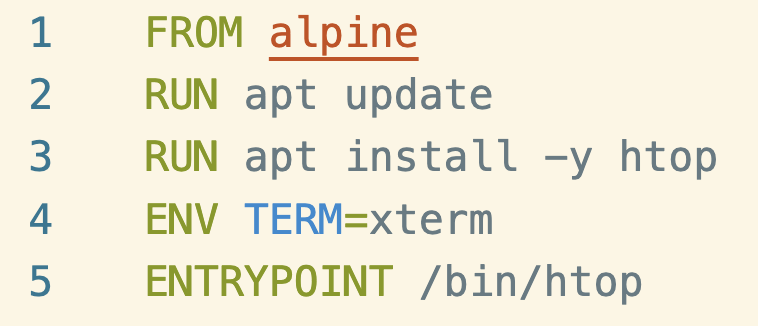
\includegraphics[scale=0.45]{images/docker_simple.png}
        \end{center}
    \end{column}
\end{columns}

La documentation complète est accessible ici: \url{https://docs.docker.com/reference/dockerfile/}

\end{frame}

% -----------------


\begin{frame}{Exemple de Dockerfile}

\begin{columns}[T,onlytextwidth]
    \begin{column}{.45\linewidth}

    \begin{itemize}
        \item \texttt{\textbf{FROM}} avec une version d'image;
        \item \texttt{\textbf{WORKDIR}} pour indiquer le dossier de travail dans lequel se placer quand le conteneur démarrera; 
        \item \texttt{\textbf{ADD}} pour ajouter des fichiers depuis la machine locale (i.e., hôte) à l'image du conteneur;
        \item \texttt{\textbf{CMD}} pour définir quelles commandes doivent être exécutées au démarrage du conteneur.
    \end{itemize}
        
    \end{column}
    \begin{column}{.5\linewidth}
        \begin{center}
            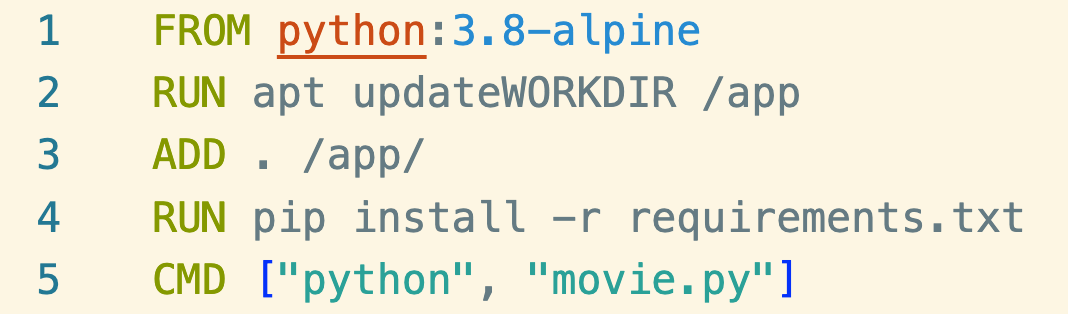
\includegraphics[scale=0.4]{images/docker_simple2.png}
        \end{center}
    \end{column}
\end{columns}
\end{frame}

\begin{frame}{Quelques subtilités des commandes Dockerfile}
\begin{itemize}
    \item \texttt{\textbf{ADD}} $\neq$ \texttt{\textbf{COPY}}: \texttt{\textbf{ADD}} fait la même chose que \texttt{\textbf{COPY}} mais permet aussi de décompresser automatiquement des archives locales, et télécharger une ressource depuis une URL
    
    \vspace{1cm}
    
    \item \texttt{\textbf{ENTRYPOINT}} $\neq$ \texttt{\textbf{CMD}}: \texttt{\textbf{ENTRYPOINT}} sert à démarrer un programme principal fixe (e.g., python, java) alors que \texttt{\textbf{CMD}} sert à remplacer les argumments passé après \texttt{\textbf{docker run image}} (e.g., \texttt{\textbf{/bin/sh}} dans le premier exemple)
\end{itemize}

\end{frame}

% -----------------

\begin{frame}{Construire une image à partir d'un Dockerfile}

\begin{block}{Commande}
\texttt{\textbf{docker build [OPTIONS] PATH}}
\end{block}

\texttt{\textbf{> docker build . -t ”monapp:latest”}}
\begin{itemize}
    \item \texttt{\textbf{docker build}} est la commande pour construire une image Docker;
    \item \texttt{\textbf{.}} est le chemin vers le Dockerfile;
    \item \texttt{\textbf{-t}} est une option pour nommer cette image (ici \texttt{\textbf{”monapp:latest”}} se réfère à un nom et une version);
    \item Par défaut, le Dockerfile est \texttt{\textbf{PATH/Dockerfile}}, mais vous pouvez donner un autre nom en utilisant l'option \texttt{\textbf{-f}}.
\end{itemize}

\end{frame}

% -----------------

\begin{frame}{Docker CLI}

\texttt{\textbf{> docker -h}} donne l'aide racine de la CLI\\
\texttt{\textbf{> docker images -h}} donne l'aide pour les images\\

\texttt{\textbf{> docker pull hello-world}} télécharge l'image \texttt{\textbf{hello-world}}\\
\texttt{\textbf{> docker images}}, ou \texttt{\textbf{ docker images ls}}, donne une liste des images téléchargées\\
\texttt{\textbf{> docker image inspect id}} donne des détail sur l'image correspondante à l'\texttt{\textbf{id}}\\

\texttt{\textbf{> docker run hello-world}} créer et démarre un conteneur à partir d'une image\\
\texttt{\textbf{> docker ps}} affiche les conteneurs en cours d'exécution\\
\texttt{\textbf{> docker ps -a}} affiche tous les conteneurs, y compris ceux aux statut \texttt{\textbf{exited}}\\
\texttt{\textbf{> docker container inspect id}} donne des détail sur le conteneur correspondant à l'\texttt{\textbf{id}}\\

\texttt{\textbf{> docker container prune}} supprime tous les conteneurs qui ne sont plus utilisés\\
\texttt{\textbf{> docker image rm hello-world}} supprime l'image locale \texttt{\textbf{hello-world}}
\end{frame}


% -----------------
\section{Quelques bonnes pratiques}
% -----------------

\begin{frame}{Penser aux couches}

Dans les versions plus anciennes de Docker, chaque ligne dans le Dockerfile créait une couche. En conséquences:
\begin{itemize}
    \item Trop de couches intermédiaires, pouvant être coûteuses;
    \item Le temps de build pouvait être impacté;
    \item Les optimisations de stockage pouvaient être impossibles;
    \item Aujourd'hui, \texttt{\textbf{RUN}}, \texttt{\textbf{COPY}} et \texttt{\textbf{ADD}} uniquement créent de nouvelles couches.
\end{itemize}

\begin{alertblock}{Bonne pratique 1}
Pensez à vos couches quand vous utiliser \texttt{\textbf{RUN}}, \texttt{\textbf{COPY}} et \texttt{\textbf{ADD}} dans votre Dockerfile
\end{alertblock}

\end{frame}

% -----------------

\begin{frame}{Réduire la taille d'une image}

\begin{alertblock}{Bonne pratique 2}
N'installez uniquement que les dépendances nécessaires dans votre Dockerfile
\end{alertblock}

\begin{itemize}
    \item Si vous utilisez \texttt{\textbf{apt}} pour installer des packages, utilisez l'option \texttt{\textbf{--no-install-recommends}}
    \item Si possible, supprimez les fichiers intermediaires non requis quand vous appliquez \texttt{\textbf{RUN}}
\end{itemize}

\end{frame}

% -----------------

\begin{frame}{Construction en plusieurs étapes}

\begin{alertblock}{Bonne pratique 3}
\begin{itemize}
    \item Réduisez la taille des images en supprimant les dépendances de compilation dans l'image finale.
    \item L'image finale contient uniquement les dépendances nécessaires à l'exécution du service.
    \item Une image de base bien adaptée aux fichiers exécutables uniquement est \texttt{\textbf{scratch}} ou \texttt{\textbf{alpine}}.
\end{itemize}
\end{alertblock}


\begin{center}
    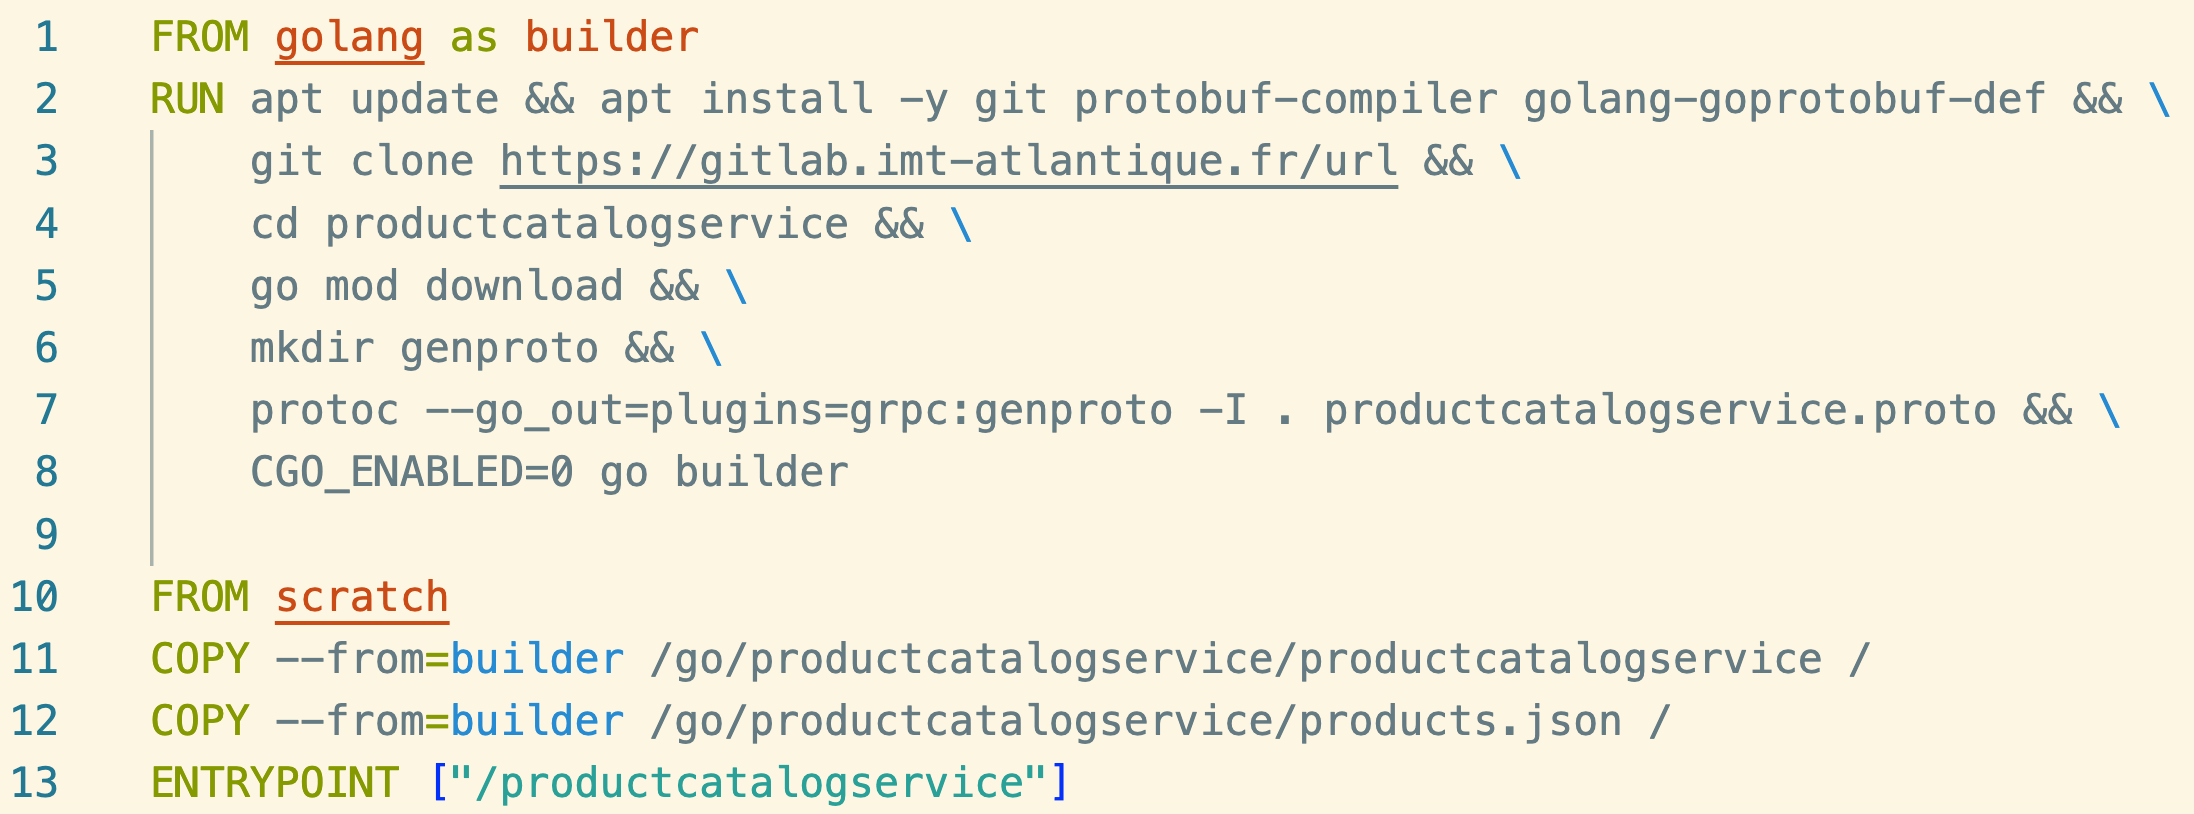
\includegraphics[scale=0.25]{images/dockerfile.png}
\end{center}

\end{frame}

% -----------------

\begin{frame}{Sécurité}
\alert{N'importe qui peut déposer une image Docker sur Docker Hub !}

\begin{alertblock}{Bonne pratique 4}
\begin{itemize}
    \item Préférez toujours les images Docker officielles.
    \item Vérifiez que l'image Docker est régulièrement mise à jour.
    \item Soyez sur que l'image contient ce que vous pensez en utilisant 
    \begin{itemize}
        \item \texttt{\textbf{> docker history image\_name}}
        \item des outils comme \texttt{\textbf{\color{blue} dive}}
    \end{itemize}
    \item Soyez sure de mettre à jour les images que vous utilisez.
\end{itemize}
\end{alertblock}

\end{frame}

% -----------------

\begin{frame}{Un peu plus dans les Dockerfiles}

\begin{itemize}
    \item Exposer ses ports dans un Dockerfile
        \begin{itemize}
            \item \texttt{\textbf{EXPOSE 80}} pour exposer un numéro de port
            \item \texttt{\textbf{EXPOSE 56/udp}} pour exposer un numéro de port pour un protocole précis
        \end{itemize}
    \vspace{0.2cm}
    \item Ajouter des données purement informatives
        \begin{itemize}
            \item \texttt{\textbf{LABEL maintainer=”Jolan PHILIPPE”}}
        \end{itemize}
    \vspace{0.2cm}
    \item Ajouter des variables d’environnement
        \begin{itemize}
            \item \texttt{\textbf{ENV ADMIN\_USER=”Alice”}}
            \item ou directement via la CLI: \texttt{\textbf{docker run -e ADMIN\_USER=”Bob”}}
        \end{itemize}
    \vspace{0.2cm}
    \item Ajouter des volumes depuis l'hôte
        \begin{itemize}
            \item \texttt{\textbf{VOLUME /myapp/data}}
        \end{itemize}
\end{itemize}


\end{frame}

% -----------------
\section{Déployer une pile logicielle avec Docker Compose }
% -----------------

\begin{frame}{Automatiser le déploiement d'applications dans des conteneurs}

\begin{center}

\includegraphics[scale=0.15]{images/docker-compose.png}
\end{center}

\begin{itemize}
    \item Déploie facilement une pile logicielle conteneurisée
    \item Défini votre déploiement avec un seul fichier YAML (conteneurs, volumes, réseaux, etc.)
    \item Les fichiers de déploiement deviennent faciles à partager, à contrôler leurs versions, etc. (c'est de l'IaC :wink:)
\end{itemize}

\end{frame}

% -----------------

\begin{frame}{Structure de \texttt{compose.yaml}}

\begin{columns}[T,onlytextwidth]
    \begin{column}{.48\linewidth}
    Spécification complète: \url{https://docs.docker.com/reference/compose-file/}
    \begin{itemize}
        \item \emph{\textbf{services}} 
        \begin{itemize}
            \item Nom du service
            \begin{itemize}
                \item \emph{\textbf{image}} Docker ou chemin de \emph{\textbf{build}} pour le Dockerfile
                \item \emph{\textbf{ports}} exposés par le service
                \item \emph{\textbf{networks}} utilisés par le service
                \item \emph{\textbf{volumes}} utilisés par le service
                \item variables d'\emph{\textbf{environment}} utilisés par le service avec sa valeur
                \item \emph{\textbf{depends\_on}} un autre service
            \end{itemize}
        \end{itemize}
        \item \emph{\textbf{volumes}} 
        \item \emph{\textbf{networks}} 
    \end{itemize}
    \end{column}
    \begin{column}{.5\linewidth}
        \vspace{-0.4cm}
        \begin{center}
            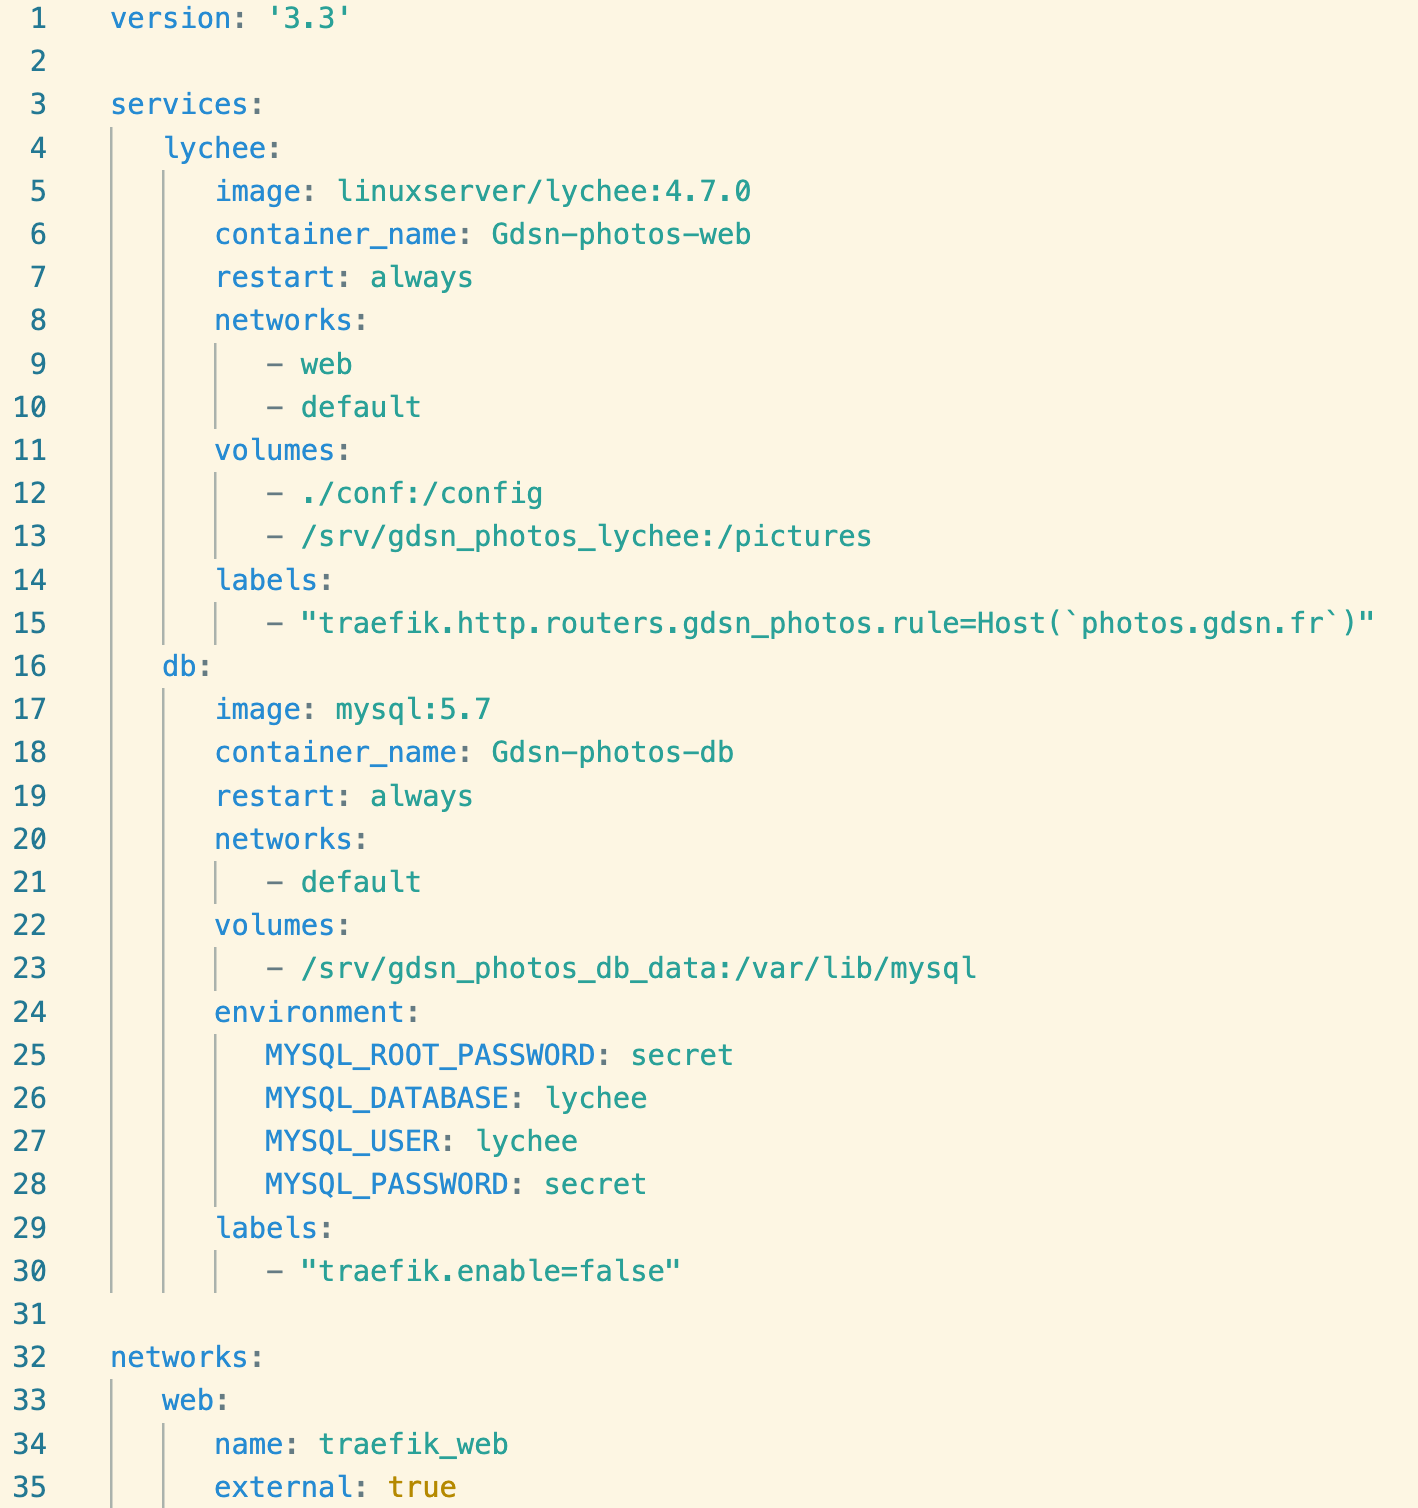
\includegraphics[scale=0.25]{images/docker_compose_code.png}
        \end{center}
    \end{column}
\end{columns}

Il est très important de comprendre que \texttt{\textbf{Docker compose}} crée un DNS pour que les conteneurs puissent s'appeler les uns les autres sans connaître leurs adresses IP.

\end{frame}

% -----------------

\begin{frame}{CLI}

Quelques commandes importantes :
\begin{itemize}
    \item \texttt{\textbf{> docker-compose build}} pour construire, ou reconstruire, des images
    \item \texttt{\textbf{> docker-compose up}} pour créer et démarrer des conteneurs, réseaux, etc.
    \item \texttt{\textbf{> docker-compose stop}} pour arrêter des conteneurs, réseaux, etc.
    \item \texttt{\textbf{> docker-compose down}} pour arrêter et supprimer des conteneurs, réseaux, etc.
\end{itemize}
        
Toute la documentation : \url{https://docs.docker.com/compose/reference/}

Quelques exemples : \url{https://github.com/docker/awesome-compose}

\end{frame}

% -----------------

\end{document}
